\begin{figure}[h!]
\centering
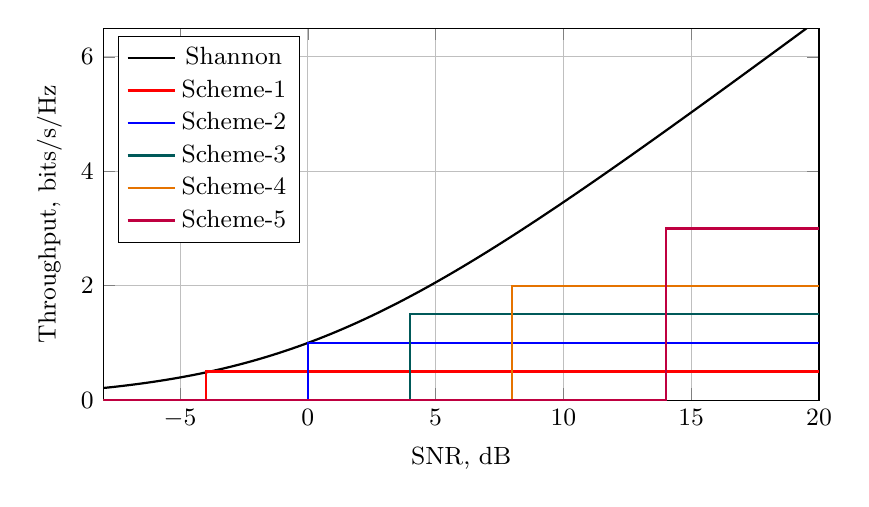
\begin{tikzpicture}
\begin{axis}[
    width=0.88\textwidth,
    height=0.52\textwidth,
    xlabel={SNR, dB},
    ylabel={Throughput, bits/s/Hz},
    xmin=-8, xmax=20,
    ymin=0, ymax=6.5,
    grid=both,
    major grid style={gray!50},
    minor grid style={gray!20},
    legend style={
        at={(0.02,0.98)},
        anchor=north west,
        fill=white,
        draw=black,
        font=\small
    },
    tick label style={font=\small},
    label style={font=\small},
    every axis plot/.append style={thick}
]

\addplot[domain=-8:20,samples=300,black]
    {ln(1 + 10^(x/10))/ln(2)};
\addlegendentry{Shannon}

\addplot[red, const plot] coordinates {(-8,0) (-4,0) (-4,0.5) (20,0.5)};
\addlegendentry{Scheme-1}

\addplot[blue, const plot] coordinates {(-8,0) (0,0) (0,1.0) (20,1.0)};
\addlegendentry{Scheme-2}

\addplot[teal!70!black, const plot] coordinates {(-8,0) (4,0) (4,1.5) (20,1.5)};
\addlegendentry{Scheme-3}

\addplot[orange!90!black, const plot] coordinates {(-8,0) (8,0) (8,2.0) (20,2.0)};
\addlegendentry{Scheme-4}

\addplot[purple, const plot] coordinates {(-8,0) (14,0) (14,3.0) (20,3.0)};
\addlegendentry{Scheme-5}

\end{axis}
\end{tikzpicture}
\caption{Throughput versus SNR for candidate schemes and Shannon bound.}
\label{fig:amc_snr_2}
\end{figure}
